\documentclass[12pt,a4paper]{article}
\usepackage[utf8]{inputenc}
\usepackage[romanian]{babel}
\usepackage{graphicx}
\usepackage{amsmath}
\usepackage{amssymb}
\usepackage{geometry}
\usepackage{hyperref}
\usepackage{listings}
\usepackage{xcolor}
\usepackage{fancyhdr}
\usepackage{float}
\usepackage{enumitem}
\usepackage{titlesec}
\usepackage{tikz}
\usepackage{setspace} % Pentru distanța dintre rânduri
\usepackage{times} % Pentru font Times New Roman
\usetikzlibrary{arrows.meta, positioning, shapes.geometric}

\geometry{
    a4paper,
    top=2.5cm,
    bottom=2.5cm,
    left=2.5cm,
    right=2.5cm
}

\hypersetup{
    colorlinks=true,
    linkcolor=blue,
    filecolor=magenta,      
    urlcolor=cyan,
}

% Stiluri pentru cod
\definecolor{codegreen}{rgb}{0,0.6,0}
\definecolor{codegray}{rgb}{0.5,0.5,0.5}
\definecolor{codepurple}{rgb}{0.58,0,0.82}
\definecolor{backcolour}{rgb}{0.95,0.95,0.92}

\lstdefinestyle{mystyle}{
    backgroundcolor=\color{backcolour},   
    commentstyle=\color{codegreen},
    keywordstyle=\color{magenta},
    numberstyle=\tiny\color{codegray},
    stringstyle=\color{codepurple},
    basicstyle=\ttfamily\footnotesize,
    breakatwhitespace=false,         
    breaklines=true,                 
    captionpos=b,                    
    keepspaces=true,                 
    numbers=left,                    
    numbersep=5pt,                  
    showspaces=false,                
    showstringspaces=false,
    showtabs=false,                  
    tabsize=2
}

\lstset{style=mystyle}

% Configurare pagina
\pagestyle{fancy}
\fancyhf{}
\setlength{\headheight}{14.5pt} % Ajustare înălțime antet
\renewcommand{\headrulewidth}{0pt} % Eliminare linie antet
\renewcommand{\footrulewidth}{0pt} % Eliminare linie subsol
\lhead{}
\rhead{}
\lfoot{}
\cfoot{\thepage}
\rfoot{}

% Configurare text
\setstretch{1.15} % Distanța dintre rânduri
\setlength{\parindent}{0pt} % Eliminare indentare paragraf
\setlength{\parskip}{6pt} % Spațiu între paragrafe

\begin{document}

\begin{titlepage}
    \centering
    \vspace*{\fill}
    {\huge\bfseries Sistem de Monitorizare Anti-Plagiat pentru Examene \par}
    \vspace*{\fill}
    \raggedright
    {\large\bfseries Autor: Pletea-Marinescu Valentin, 332AB \par}
    {\large\bfseries An: 2024-2025 \par}
\end{titlepage}

% Cuprins
\tableofcontents
\newpage

\section{Introducere}

\subsection{Contextul și relevanța temei}

Plagiatul reprezintă una dintre problemele grave ale sistemului de
învățământ, iar, de când cu apariția și dezvoltarea inteligenței
artificiale, lucrurile s-au accentuat. Alegerea acestei teme constă în
oportunitatea de a oferi șanse egale tuturor participanților, în
cadrul unui examen, iar acest sistem de anti-plagiat, propus în acest
proiect, reprezintă o soluție inovatoare, prin combinarea tehnicilor
moderne de computer vision și inteligență artificială, care își
propune să monitorizeze comportamentului candidaților și de a semnala
posibile tentative de fraudă.

Conform studiului realizat de Gabriela Pelican \cite{pelican}, plagiatul
afectează absolut toate nivelurile educaționale, iar, în cazul
României, lucrurile nu merg foarte bine la capitolul acesta, autoarea
menționând că ``România prezintă cea mai ridicată rată a plagiatelor
descoperite pe tărâmul Uniunii, și anume 26.1\% din totalitatea
operelor verificate, valoare aproape dublă în comparație cu media
europeană , precum și aceea că incidența cazurilor de plagiat este cu
mult mai ridicată în statele din regiunea estică a Europei, țări ale
căror niveluri de trai și de educație sunt considerabil inferioare
raportat la țările vestice.''

De asemenea, un alt studiu \cite{science}, publicat de cei de la Science, ne
relatează că România este țara cu cel mai mare număr de articole
științifice eliminate din cuprinsul publicațiilor de specialitate ca
urmare a nerespectării normelor de conduită în cercetarea științifică,
prin raportare la totalul fondurilor alocate pentru cercetare și de
asemenea, ocupă locul secund în topul țărilor cu cel mai mare număr de
articole retrase raportat la totalul articolelor publicate, în urma
descoperirii plagierii.

\subsection{Obiectivele proiectului}

Acest proiect își propune să ofere un sistem inovator pentru monitorizarea examenelor, cu următoarele obiective specifice:

\begin{enumerate}[label=\arabic*.]
    \item \textbf{Detecția privirii candidatului:} Semnalarea și înregistrarea situațiilor
    în care candidatul privește în alte direcții precum stânga, dreapta sau jos, 
    decât în propriul ecran al monitorului sau în propria foaie, în cazul unui examen scris.
    
    \item \textbf{Identificarea obiectelor neautorizate:} Detectarea dispozitivelor precum
    smartwatch sau telefon, care pot fi folosite pentru a obține informații, 
    ceea ce ar duce la fraudarea respectivului examen.
    
    \item \textbf{Înregistrare și arhivare:} Realizarea unei înregistrări video în care 
    vor fi capturate și arhivate sesiunile de examen pentru o analiză ulterioară, 
    evidențiind tentativele probabile de fraudă.
    
    \item \textbf{Generarea rapoartelor:} Crearea rapoartelor detaliate în formate html, csv și json,
    contribuind astfel la o analiză mai clară și mai sigură pentru evaluatori.
    
    \item \textbf{Interfață intuitivă:} Dezvoltarea unei interfețe grafice intuitive, care să permită
    supraveghetorilor utilizarea tuturor funcționalităților menționate anterior.
\end{enumerate}

\subsection{Avantajele abordării propuse}

În general, multe soluții de combatere a plagiatului se concentrează mai mult 
pe monitorizarea ecranului candidatului, dar acest sistem este centrat pe 
comportamentul fizic al acestuia. Consider că, prin urmărirea direcției privirii 
și detectarea obiectelor neautorizate, sistemul poate identifica indicii ale
comportamentului fraudulos, oferind dovezi concrete care pot fi analizate ulterior. 
Acest lucru poate contribui semnificativ la menținerea integrității academice, 
fără a mai fi nevoie să se creeze acea atmosferă de supraveghere excesivă.

Este normal ca respectivul sistem să ofere, pe lângă rezultatele
remarcabile, și falsuri-pozitive, din cauza unor factori precum
iluminarea sălii de examen sau mișcări naturale ale capului, fară
intenția de a privi în altă direcție. Astfel, prin intermediul
funcționalităților de înregistrare video și semnalare în timp real al
comportamentelor posibil frauduloase, poate să existe, după terminarea
respectivului examen, o discuție între profesor și student pe baza
onestității sale și de a ajunge la rezultatul final. 

Tehnologia avansează pe zi ce trece, iar diversele tentative de plagiat se diversifică automat.
Așadar, este absolut firesc ca și sistemele care încearcă, prin
diverse mijloace, să combată fraudarea examenelor, să avanseze și ele.

\section{Analiza domeniului și soluții existente}

\subsection{Soluții similare existente pe piață}

Au apărut pe piață, de-a lungul timpului, diferite soluții de
monitorizare și combatere a fraudei în cadrul examenelor. În urma cercetării, am identificat
trei sisteme principale care propun soluții similare cu acest proiect: ProctorU \cite{proctoru}, 
Proctorio \cite{proctorio} și Respondus Lockdown Browser \cite{respondus}.

\subsubsection{ProctorU}
ProctorU este una dintre cele mai utilizate platforme în
supravegherea examenelor online. Se bazează atât pe monitorizarea
ecranului candidatului, cât și pe comportamentul acestuia. 

\begin{table}[h]
\centering
\begin{tabular}{|p{7.5cm}|p{7.5cm}|}
\hline
\textbf{Puncte forte} & \textbf{Limitări} \\
\hline
\begin{itemize}
    \item Verificarea identității candidatului prin legitimație sau act de identitate
    \item Supravegherea umană în timp real
    \item Monitorizarea completă a activității pe calculator
    \item Detectarea comportamentului suspect prin AI
\end{itemize} & 
\begin{itemize}
    \item Costuri ridicate (15-25 USD per candidat)
    \item Necesită conexiune stabilă la internet
    \item Mai puțin adecvat pentru examenele fizice
    \item Probleme potențiale de confidențialitate
\end{itemize} \\
\hline
\end{tabular}
\caption{Analiza comparativă a sistemului ProctorU}
\end{table}

Platforma înregistrează fiecare secundă, se asigură că nu există alte tab-uri
deschise, cu excepția aceluia în care se susține respectivul examen,
nu permite anumite combinații de taste din tastatură pentru funcții precum 
print, copy sau paste și, prin intermediul unei camere web, platforma poate 
supraveghea candidatul eficient.

\subsubsection{Proctorio}
Un alt sistem similar este Proctorio, asemănător cu
ProctorU, dar care este complet automatizat, întrucât se bazează doar
pe tehnologii de AI și machine learning pentru detectarea posibilelor
tentative de fraudă, fără a mai avea nevoie de asistență umană.

\begin{table}[h]
\centering
\begin{tabular}{|p{8.5cm}|p{8.5cm}|}
\hline
\textbf{Puncte forte} & \textbf{Limitări} \\
\hline
\begin{itemize}
    \item Instalare și configurare simplă prin extensie browser
    \item Funcționalități de blocare a navigării web
    \item Algoritmi care reduc necesitatea intervenției umane
    \item Costuri mai reduse decât ProctorU
\end{itemize} & 
\begin{itemize}
    \item Rată ridicată de falsuri-pozitive
    \item Dificultate în detectarea utilizării dispozitivelor secundare
    \item Funcționează doar pe Google Chrome
    \item Probleme de confidențialitate
\end{itemize} \\
\hline
\end{tabular}
\caption{Analiza comparativă a sistemului Proctorio}
\end{table}

Monitorizarea se bazează pe recunoaștere facială, analizând comportamentul prin 
intermediul mișcării capului sau a ochilor. Sistemul se ocupă și de monitorizarea 
ecranului, observă dacă există alte tab-uri deschise și dacă sunt pornite în fundal 
aplicații care ar putea facilita fraudarea examenului.

\subsubsection{Respondus Lockdown Browser}
Respondus Lockdown Browser reprezintă o abordare diferită, 
întrucât se concentrează pe crearea unui mediu securizat pentru examen,
prin blocarea accesului candidatului la alte aplicații și resurse.

Conform documentației sale oficiale~\cite{respondus}, această soluție se
integrează cu sisteme de management al învățării (LMS), precum Canvas,
Blackboard, Moodle, Schoology și Brightspace.

\begin{table}[H] % Changed from [h] to [H] to force table placement
    \centering
    \begin{tabular}{|p{8.5cm}|p{8.5cm}|}
    \hline
    \textbf{Puncte forte} & \textbf{Limitări} \\
    \hline
    \begin{itemize}
        \item Împiedicarea accesului la alte programe și resurse
        \item Integrare bună cu platforme educaționale (LMS)
        \item Costuri mai reduse comparativ cu alte soluții
        \item Ușor de implementat la nivel instituțional
    \end{itemize} & 
    \begin{itemize}
        \item Incapacitatea de a detecta dispozitive secundare
        \item Nu monitorizează comportamentul fizic al candidatului
        \item Funcționalitate restrânsă pe dispozitivele mobile
        \item Incompatibilitate cu programe specifice (IDE-uri, etc.)
    \end{itemize} \\
    \hline
    \end{tabular}
    \caption{Analiza comparativă a sistemului Respondus Lockdown Browser}
\end{table}

\subsection{Aspecte multimedia relevante}

\subsubsection{Protocoale și transmisie de date}
În cadrul aspectelor legate de multimedia, întâlnim protocoale care
asigură transmisia datelor sigură și optimizată:
\begin{itemize}
    \item \textbf{WebRTC} pentru comunicația audio-video în timp real. Acest protocol este utilizat pentru a transmite fluxul video capturat de la webcam către sistemul de procesare, asigurând o latență minimă și o calitate optimă a transmisiei. În proiectul nostru, WebRTC este folosit pentru a permite monitorizarea în timp real a candidaților, oferind o conexiune stabilă și eficientă.
    \item \textbf{TLS/SSL} pentru criptarea întregului flux de date. Acest strat de securitate este esențial pentru a proteja datele transmise între client și server, prevenind accesul neautorizat sau interceptarea informațiilor sensibile. În contextul proiectului nostru, TLS/SSL este utilizat pentru a securiza atât fluxul video, cât și datele generate, cum ar fi rapoartele de încălcări.
\end{itemize}

\subsubsection{Procesare video și audio}
În ceea ce privește procesarea video, fluxul capturat de la webcam este procesat în
timp real pentru a detecta comportamente suspicioase. Se utilizează algoritmi de
compresie video standard, precum \textbf{H.264}, pentru a asigura transmisia
eficientă a datelor, reducând în același timp latența și consumul de
bandă. În proiectul nostru, H.264 este utilizat pentru a comprima fluxul video înainte de stocare sau transmitere, asigurând o utilizare eficientă a resurselor hardware.

Platformele de monitorizare înregistrează și sunetele de pe fundal, analizând 
eventuale conversații sau zgomote suspecte. Se aplică algoritmi de compresie audio, 
precum \textbf{AAC} sau \textbf{Opus}, pentru transmiterea fluxului audio în timp real. În proiectul nostru, aceste algoritmi sunt folosiți pentru a înregistra și analiza sunetele de fundal, oferind informații suplimentare despre posibilele încălcări.

\subsubsection{Watermarking și steganografie}
În soluțiile de tip Lockdown Browser se aplică watermark-uri vizibile sau invizibile 
asupra conținutului afișat pe ecran, având ca scop prevenirea capturării neautorizate 
a informațiilor de examen. În proiectul nostru, watermark-urile sunt utilizate pentru a marca fluxul video înregistrat cu informații precum timestamp-ul și ID-ul candidatului, asigurând autenticitatea și integritatea datelor.

De asemenea, steganografia (metoda de ascundere a informațiilor 
într-un conținut media) este utilizată pentru a insera metadate în fluxul video, fără a afecta calitatea vizuală. Aceste metadate includ informații despre sesiunea de monitorizare, cum ar fi locația camerei sau setările de procesare, și pot fi extrase ulterior pentru verificări suplimentare.

\subsubsection{Sincronizarea datelor multimedia}
Pentru a asigura o corelare precisă între fluxul video, audio și evenimentele detectate, proiectul nostru utilizează timestamp-uri sincronizate. Aceste timestamp-uri sunt generate în momentul capturării fiecărui cadru video sau pachet audio și sunt utilizate pentru a lega alertele generate de sistem cu momentul exact al încălcării. Această abordare permite o analiză detaliată și o verificare ulterioară eficientă.

\subsubsection{Optimizări pentru hardware limitat}
Pentru a permite rularea eficientă a sistemului pe dispozitive cu resurse hardware limitate, proiectul nostru implementează mai multe optimizări:
\begin{itemize}
    \item Procesarea unui cadru din 20 pentru detectarea obiectelor, reducând astfel consumul de resurse.
    \item Utilizarea unui buffer circular pentru gestionarea eficientă a cadrelor video.
    \item Integrarea unui sistem de cache pentru alertele generate, evitând duplicarea mesajelor de alertă.
\end{itemize}
Aceste optimizări asigură o performanță ridicată, chiar și pe hardware obișnuit, fără a compromite acuratețea detecției.

\subsection{Avantajele soluției propuse față de cele existente}

Sistemul de monitorizare anti-plagiat propus în acest proiect aduce următoarele avantaje față de soluțiile existente:

\begin{enumerate}
    \item \textbf{Focalizare pe comportamentul fizic} - Spre deosebire de soluțiile existente care se concentrează predominant pe monitorizarea ecranului, sistemul nostru pune accent pe comportamentul fizic al candidatului.
    
    \item \textbf{Detecție specializată a obiectelor} - Utilizăm tehnologii avansate de computer vision pentru a detecta dispozitive neautorizate (telefoane, smartwatch-uri), aspect în care Respondus Lockdown Browser prezintă limitări importante.
    
    \item \textbf{Rapoarte comprehensive} - Generarea automată a rapoartelor în multiple formate (HTML, CSV, JSON) facilitează analiza ulterioară și documentarea incidentelor.
    
    \item \textbf{Fără dependență de browser} - Spre deosebire de Proctorio care funcționează doar pe Google Chrome, aplicația noastră este independentă de browser.
    
    \item \textbf{Costuri reduse} - Implementarea locală reduce semnificativ costurile per candidat comparativ cu soluțiile precum ProctorU.
\end{enumerate}

\section{Implementarea propriu-zisă}

În cadrul implementării sistemului de anti-plagiat, a fost necesară utilizarea mai multor biblioteci specializate, fiecare având un rol diferit în funcționarea sa.

\subsection{OpenCV}
Am utilizat biblioteca OpenCV (\texttt{Open Source Computer Vision Library}),
care a avut un rol principal în prelucrarea și procesarea imaginilor. Cu
ajutorul ei, am captat fluxul video de la camera web, prin intermediul
funcției \texttt{VideoCapture}, care joacă rolul de interfață primară cu lumea
fizică, capturând imaginile candidatului care sunt apoi analizate pentru
a detecta comportamente suspecte.

Această bibliotecă mi-a oferit funcția \texttt{cvtColor}, cu care am reușit să
transform imaginile color în tonuri de gri, ceea ce a dus la o eficiență
mult mai mare pe partea de detectare facială, deoarece reduce
complexitatea computațională, făcând referire doar la o singură valoare
pentru fiecare pixel, în loc de trei, și îmbunătățește performanțele
algoritmilor de analiză a imaginii, care adesea funcționează mai bine cu
imagini în tonuri de gri.

În cadrul detecției precise al pupilelor, am aplicat un filtru gaussian,
cu scopul de a reduce zgomotul din imagini, apelând funcția
\texttt{cv2.GaussianBlur}, oferită de respectiva bibliotecă, care este un filtru
esențial în procesarea imaginilor. Parametrii acestei funcții sunt
imaginea sursă, fiind regiunea izolată a ochiului, dimensiunea
kernel-ului, în cazul nostru fiind de 7x7, deoarece s-a constatat, după
mai multe teste, că oferă cele mai bune rezultate pentru detectarea
pupilelor și este suficient de mare pentru a acoperi variațiile minore
de intensitate din jurul pupilei, în comparație cu kernel-uri mai mici
de 3x3 sau 5x5, care păstrează prea multe detalii fine și zgomot sau
kernel-uri prea mari de 9x9 sau 11x11, care estompează prea mult
imaginea, ducând la pierderea marginii pupilei și deviația standard a
distribuției Gaussiene, acest parametru fiind setat la valoarea 0,
însemnând că este calculată automat, folosind formula:

\begin{equation}
\sigma = 0.3 \cdot \left( \frac{\texttt{kernel\_size} - 1}{2} - 1 \right) + 0.8
\end{equation}

\hspace{-6mm}Pentru un kernel de dimensiune \(7 \times 7\), această formulă devine:
\begin{align}
\sigma &= 0.3 \cdot \left( \frac{7 - 1}{2} - 1 \right) + 0.8 \nonumber \\
    &= 0.3 \cdot (3 - 1) + 0.8 \nonumber \\
    &= 0.3 \cdot 2 + 0.8 \nonumber \\
    &= 1.4
\end{align}

Funcția \texttt{cv2.minMaxLoc} din OpenCV este un instrument esențial pentru
detecția pupilelor. Această funcție identifică valorile minime și maxime
dintr-o imagine, împreună cu coordonatele acestora. Ea retunează patru
valori: valoarea minimă, valoarea maximă, coordonatele valorii minime și
coordonatele valorii maxime. În cazul nostru, valoarea de interes este
reprezentată de coordonatele valorii minime, deoarece reprezintă cel mai
întunecat punct din regiunea ochiului, iar pupila este tipic cea mai
întunecată parte a ochiului, deci această abordare eficientă permite
localizarea rapidă a centrului pupilei. Această metodă funcționează
deoarece, înainte de a aplica \texttt{minMaxLoc}, imaginea este pre-procesată de
acel filtru gaussian, menționat mai sus, care reduce zgomotul și
uniformizează valorile, făcând detectarea mai robustă la variații minore
în iluminare sau textura irisului.

Tot cu ajutorul lui OpenCV, am reușit să desenez elemente vizuale
sugestive, cum ar fi dreptunghiuri în zona obiectelor detectate,
folosind funcția \texttt{cv2.rectangle()}, și să afișez text pentru alerte,
folosind \texttt{cv2.putText()}, iar salvarea și comprimarea înregistrărilor a
fost realizată folosind \texttt{VideoWriter}.

De asemenea, am reușit să creez o mască, pentru a izola obiectul de
interes, precum ochiul, utilizând funcții precum \texttt{fillPoly} și
\texttt{bitwise\_not}. Funcția \texttt{cv2.fillPoly} umple o zonă poligonală într-o imagine
cu o culoare specifică, iar, în contextul acestui sistem, este folosită
pentru a crea o mască pentru izolarea regiunii ochilor. Primește ca
parametrii imaginea pe care se desenează, un array de puncte care
definesc poligonul, în cazul nostru fiind vorba de conturul ochiului, și
culoarea de umplere, spre exemplu (0, 0, 0), care în RGB înseamnă
culoare negru. Astfel, rezultatul este o mască în care regiunea ochiului
este colorată în negru, iar restul imaginii rămâne alb.

Funcția \texttt{cv2.bitwise\_not} inversează valorile de bit ale fiecărui pixel
din imagine, fiind echivalentă cu operația de negare bitwise ($\sim$). Am
folosit-o pentru a inversa masca creată, astfel încât regiunea ochiului
să fie izolată din restul imaginii. Această funcție primește ca
parametrii imaginea sursă și o mască opțională care determină pe ce
regiune se aplică operația. Astfel, aceste două funcții lucrează
împreună pentru a crea o ``tăietură'' precisă a regiunii ochiului, din
întreaga imagine, pentru a analiza foarte precis pupila, fără
interferențe din alte părți ale imaginii.

Funcția \texttt{cv2.circle} din OpenCV desenează un cerc pe o imagine, astfel eu
mă folosesc de aceasta, pentru evidențierea vizuală a pupilelor
detectate. Marchez poziția pupilelor detectate pe imagine, le evidențiez
utilizând culori diferite pentru a indica starea, precum verde pentru
privire centrată sau roșu pentru privire suspectă, și ofer în același
timp și un feedback vizual pentru supraveghetor, în ceea ce privește
direcția privirii candidatului. Ca și parametrii, funcția primește
imaginea pe care se desenează respectivul cerc, coordonatele centrului
cercului, în cazul nostru al centrului pupilei, raza cercului, culoarea
și grosimea liniei, dar, pentru grosime, am utilizat valoarea -1,
deoarece am vrut un cerc plin.

Așadar, biblioteca OpenCV este responsabilă pentru tot ce înseamnă ``a
vedea'' în acest sistem.

\subsection{Dlib}
Biblioteca Dlib a fost utilizată pentru detectarea feței și extragerea reperelor faciale \cite{dlib}. Aceasta a fost esențială pentru analiza privirii și determinarea direcției acesteia. 

Funcția \texttt{dlib.get\_frontal\_face\_detector} a fost utilizată pentru a inițializa detectorul de fețe bazat pe HOG (Histogram of Oriented Gradients), care s-a dovedit eficient chiar și în condiții de iluminare variabilă. Acest algoritm funcționează prin împărțirea imaginii în celule mici și calcularea gradientului de intensitate pentru fiecare celulă. Gradientul este apoi normalizat pentru a reduce efectele variațiilor de iluminare, iar rezultatul este un descriptor robust care poate fi utilizat pentru a detecta fețele în imagine. Detectorul returnează coordonatele dreptunghiurilor care încadrează fețele detectate, iar aceste coordonate sunt utilizate pentru a izola regiunea feței.

Predictorul de repere faciale a fost încărcat cu ajutorul funcției \texttt{dlib.shape\_predictor}, care a permis identificarea celor 68 de puncte de pe față. Acest predictor utilizează un model preantrenat bazat pe regresie, care estimează pozițiile punctelor faciale pe baza caracteristicilor extrase din imagine. Dintre cele 68 de puncte, punctele 36-47 au fost utilizate pentru a izola regiunea ochilor. Aceste puncte sunt distribuite astfel încât să încadreze conturul ochilor, permițând izolarea precisă a regiunii de interes.

Funcția \texttt{shape.part} a fost utilizată pentru a accesa coordonatele fiecărui punct facial, iar aceste coordonate au fost folosite pentru a calcula raporturile orizontale și verticale ale privirii. De exemplu, raportul orizontal este calculat ca raportul dintre distanța dintre pupile și lățimea ochilor, iar raportul vertical este calculat ca raportul dintre înălțimea ochilor și lățimea acestora. Aceste raporturi sunt utilizate pentru a determina direcția privirii, cum ar fi privirea spre stânga, dreapta, sus sau jos.

De asemenea, aceste puncte au fost utilizate pentru a determina orientarea capului, prin calcularea distanțelor dintre punctele cheie, cum ar fi ochii, nasul și gura. Orientarea capului este estimată prin compararea acestor distanțe cu valorile de referință, iar rezultatul este utilizat pentru a detecta mișcările capului care pot indica comportamente suspecte.

\subsection{PyTorch și YOLOv8}
Pentru detectarea obiectelor interzise, precum telefoanele mobile și smartwatch-urile, am utilizat biblioteca PyTorch \cite{pytorch} și modelul YOLOv8 dezvoltat de Ultralytics \cite{ultralytics}. 

Funcția \texttt{torch.load} a fost utilizată pentru a încărca modelele YOLOv8 preantrenate. Aceste modele sunt bazate pe arhitectura YOLO (You Only Look Once), care este optimizată pentru detectarea rapidă și precisă a obiectelor în imagini. YOLOv8 utilizează o rețea neuronală convoluțională care împarte imaginea în grile și prezice simultan clasele obiectelor și coordonatele acestora. Această abordare permite detectarea în timp real, chiar și pe dispozitive cu resurse limitate.

Metoda \texttt{model.predict} a fost folosită pentru a detecta obiectele în cadrul video. Modelul a fost configurat să proceseze doar un cadru din 20 pentru a economisi resurse și să detecteze doar categoriile de interes. Această optimizare reduce semnificativ consumul de procesor și memorie, permițând rularea eficientă a aplicației pe hardware obișnuit.

Pentru a reduce falsurile pozitive, am utilizat două modele YOLOv8 separate: unul pentru detectarea telefoanelor și altul pentru smartwatch-uri. Această abordare a permis clasificarea precisă a obiectelor detectate, chiar și în condiții de iluminare slabă sau când obiectele erau parțial vizibile. De exemplu, modelul pentru telefoane a fost antrenat să recunoască formele și dimensiunile tipice ale telefoanelor mobile, iar modelul pentru smartwatch-uri a fost antrenat să detecteze dispozitivele purtabile pe încheietura mâinii.

Funcția \texttt{model.detect} a fost utilizată pentru a genera coordonatele obiectelor detectate, iar aceste coordonate au fost utilizate pentru a desena dreptunghiuri în jurul obiectelor și pentru a genera alerte în timp real. De asemenea, coordonatele au fost utilizate pentru a calcula distanțele dintre obiectele detectate și alte elemente din imagine, cum ar fi fața candidatului, pentru a determina dacă obiectele sunt utilizate în mod activ.

\subsection{NumPy}
Biblioteca NumPy a fost utilizată pentru manipularea matricilor și a datelor numerice \cite{numpy}. 

Funcția \texttt{np.zeros} a fost folosită pentru a crea măști pentru regiunile de interes din imagine, iar \texttt{np.full} a fost utilizată pentru a inițializa matrici cu valori constante. Aceste funcții sunt esențiale pentru preprocesarea imaginilor, deoarece permit izolarea regiunilor de interes și aplicarea de operații specifice doar asupra acestor regiuni.

Funcțiile \texttt{np.min} și \texttt{np.max} au fost utilizate pentru a determina limitele regiunilor de decupat, iar operațiile vectoriale au permis calcularea rapidă a coordonatelor pupilelor și a raporturilor orizontale și verticale. De exemplu, coordonatele pupilelor sunt calculate ca punctele cu intensitatea minimă din regiunea ochilor, iar raporturile sunt calculate ca raporturi între distanțele dintre aceste coordonate și dimensiunile regiunii.

\subsection{Biblioteca datetime}
Biblioteca \texttt{datetime}\cite{datetime} din Python a fost utilizată pentru gestionarea timpului și a timestamp-urilor în cadrul proiectului. Aceasta a fost esențială pentru sincronizarea evenimentelor, generarea rapoartelor și înregistrarea timpului de monitorizare.

Funcția \texttt{datetime.now()} a fost utilizată pentru a obține timpul curent în momentul generării unui eveniment, cum ar fi detectarea unei încălcări sau salvarea unui raport. Timestamp-urile generate sunt utilizate pentru a lega evenimentele detectate de momentele exacte din fluxul video.

De exemplu, în cadrul clasei \texttt{ViolationMonitor}, funcția \texttt{datetime.now().strftime()} a fost utilizată pentru a formata timestamp-urile într-un format ușor de citit, cum ar fi \texttt{YYYY-MM-DD HH:MM:SS}. Aceste timestamp-uri sunt incluse în rapoartele generate și sunt utilizate pentru a analiza comportamentul candidatului în timp.

Funcția \texttt{timedelta} a fost utilizată pentru a calcula diferențele de timp între evenimente. De exemplu, timpul scurs de la începutul înregistrării este calculat utilizând \texttt{datetime.now()} și timpul de start al înregistrării. Acest lucru este afișat în interfața grafică pentru a oferi utilizatorului informații în timp real despre durata monitorizării.

De asemenea, biblioteca \texttt{datetime} a fost utilizată pentru a genera nume unice pentru fișierele de înregistrare și rapoarte, utilizând funcția \texttt{strftime()} pentru a include timestamp-uri în numele fișierelor.

Biblioteca \texttt{datetime} a fost astfel un instrument esențial pentru gestionarea timpului în toate aspectele proiectului, de la monitorizare în timp real până la generarea rapoartelor detaliate.

\subsection{Biblioteca logging}
Biblioteca \texttt{logging}\cite{logging} din Python a fost utilizată pentru gestionarea mesajelor de jurnalizare (\textit{logging}) în cadrul proiectului. Aceasta a fost esențială pentru monitorizarea funcționării aplicației, diagnosticarea problemelor și păstrarea unui istoric al evenimentelor importante.

Funcția \texttt{logging.basicConfig()} a fost utilizată pentru a configura formatul și nivelul de jurnalizare. În cadrul proiectului, mesajele de jurnalizare sunt salvate atât într-un fișier (\texttt{sistem\_anti\_plagiat.log}), cât și afișate în consolă. Acest lucru permite o monitorizare eficientă a aplicației în timp real, precum și o analiză ulterioară a problemelor.

De exemplu, în cadrul clasei \texttt{SistemAntiPlagiat}, biblioteca \texttt{logging} a fost utilizată pentru a înregistra evenimente importante, cum ar fi pornirea înregistrării video, detectarea încălcărilor sau erorile apărute în timpul procesării.

Biblioteca \texttt{logging} a fost utilizată și pentru a înregistra excepțiile apărute în timpul rulării aplicației, utilizând funcția \texttt{logger.exception()}, care include automat detaliile despre excepție în mesajul de jurnalizare.

Această abordare a permis identificarea rapidă a problemelor și îmbunătățirea stabilității aplicației. Biblioteca \texttt{logging} a fost astfel un instrument esențial pentru gestionarea mesajelor de jurnalizare în toate modulele proiectului.

\subsection{PyQt5}
Pentru dezvoltarea interfeței grafice, am utilizat biblioteca PyQt5 \cite{pyqt5}. Aceasta a permis crearea unei interfețe intuitive și funcționale, utilizând următoarele componente principale:

\begin{itemize}
    \item \textbf{QPushButton:} Am folosit acest widget pentru a crea butoane interactive, cum ar fi cele pentru pornirea monitorizării, înregistrării sau exportarea rapoartelor. Aceste butoane sunt esențiale pentru a permite utilizatorului să interacționeze cu aplicația într-un mod simplu și direct. De exemplu, butonul de export al raportului oferă o funcționalitate clară și accesibilă pentru utilizator.

    \item \textbf{QTextEdit:} Acest widget este utilizat pentru afișarea în timp real a rapoartelor generate. Este o alegere potrivită deoarece permite afișarea unui text formatat și poate fi setat ca "read-only", astfel încât utilizatorul să nu poată modifica conținutul raportului.

    \item \textbf{QTimer:} Timer-ul este folosit pentru actualizarea periodică a timpului de înregistrare. Aceasta este o soluție eficientă pentru a menține interfața sincronizată cu procesele din fundal, cum ar fi monitorizarea în timp real.

    \item \textbf{QLabel:} Am utilizat QLabel pentru afișarea informațiilor importante, cum ar fi numărul de încălcări detectate sau timpul de înregistrare. QLabel este ideal pentru afișarea textului static sau dinamic, fiind ușor de actualizat în funcție de starea aplicației.

    \item \textbf{QCheckBox:} Checkbox-ul pentru activarea sau dezactivarea modului de oglindire a imaginii este o alegere intuitivă. Acesta permite utilizatorului să personalizeze modul în care este afișat fluxul video, ceea ce poate fi util în funcție de preferințele sau nevoile acestuia.

    \item \textbf{QGroupBox și Layout-uri (QVBoxLayout, QHBoxLayout):} Acestea sunt folosite pentru organizarea logică a elementelor din interfață. De exemplu, gruparea statisticilor sau a controalelor într-un QGroupBox ajută la crearea unei interfețe mai clare și mai structurate. Layout-urile verticale și orizontale sunt esențiale pentru aranjarea componentelor într-un mod responsiv și estetic.

    \item \textbf{QMainWindow:} Am utilizat această clasă ca fereastră principală a aplicației. Este o alegere standard pentru aplicațiile complexe, deoarece oferă suport pentru meniuri, bare de instrumente și alte elemente avansate.

    \item \textbf{QMessageBox:} Pentru afișarea mesajelor de confirmare sau eroare, QMessageBox este o soluție simplă și eficientă. Acesta permite comunicarea clară cu utilizatorul în momente critice, cum ar fi confirmarea exportului unui raport sau notificarea unei erori.
\end{itemize}

Interfața a fost proiectată pentru a fi intuitivă și ușor de utilizat, oferind acces rapid la toate funcționalitățile sistemului.

\subsection{Modularizarea si structura proiectului}

\hspace{6mm}Proiectul a fost organizat modular, fiecare fișier Python având un rol bine definit. Această abordare facilitează întreținerea codului, testarea și extinderea funcționalităților. Mai jos sunt detaliate principalele module și responsabilitățile acestora:

\begin{itemize}
    \item \textbf{main.py:} Acesta este punctul de intrare al aplicației. Inițializează componentele principale, cum ar fi detectorul de fețe, detectorul de obiecte, monitorul de încălcări și handler-ul video. De asemenea, gestionează procesarea cadrelor și exportul rapoartelor.

    \item \textbf{gui\_app.py:} Conține implementarea interfeței grafice utilizând biblioteca PyQt5. Include funcționalități precum pornirea monitorizării, înregistrarea video, afișarea alertelor în timp real și exportul rapoartelor.
    
    \item \textbf{test\_camera.py:} Un script auxiliar pentru testarea funcționalității camerei web. Verifică dacă camera poate fi accesată și dacă fluxul video este disponibil.

    \item \textbf{modules/face\_detector.py:} Acest modul implementează detectarea feței și analiza direcției privirii utilizând biblioteca Dlib. Este responsabil pentru identificarea feței și determinarea direcției privirii candidatului.

    \item \textbf{modules/object\_detector.py:} Conține implementarea pentru detectarea obiectelor interzise, cum ar fi telefoanele mobile și smartwatch-urile, utilizând modelul YOLOv8. Este optimizat pentru procesarea eficientă a cadrelor.

    \item \textbf{modules/video\_handler.py:} Gestionează procesarea și afișarea cadrelor video. Include funcționalități pentru oglindirea imaginii, afișarea alertelor și salvarea înregistrărilor video.

    \item \textbf{modules/violation\_monitor.py:} Monitorizează încălcările detectate, cum ar fi privirea suspectă sau utilizarea obiectelor interzise. Înregistrează alertele și le sincronizează cu timestamp-uri.

    \item \textbf{modules/report\_generator.py:} Este responsabil pentru generarea rapoartelor în formate HTML, CSV și JSON. Aceste rapoarte includ detalii despre încălcările detectate și statistici generale.

    \item \textbf{modules/data\_exporter.py:} Gestionează exportul datelor în formatele specificate (CSV, JSON). Este utilizat pentru a salva informațiile despre încălcări într-un mod structurat.
    
    \item \textbf{modules/gaze\_tracking/gaze\_tracker.py:} Acest fișier implementează logica principală pentru urmărirea privirii. Utilizează reperele faciale pentru a calcula raporturile orizontale și verticale ale privirii și pentru a determina direcția acesteia.

    \item \textbf{modules/gaze\_tracking/eye.py:} Acest modul izolează regiunea ochilor din imagine și detectează pupilele. De asemenea, calculează raportul de clipire pentru a identifica dacă ochiul este închis.

    \item \textbf{modules/gaze\_tracking/pupil.py:} Acest fișier implementează logica pentru detectarea și analiza pupilelor, utilizând coordonatele și dimensiunile acestora pentru a determina starea ochilor.

    \item \textbf{requirements.txt:} Acest fișier conține lista tuturor bibliotecilor și pachetelor necesare pentru rularea aplicației. Este utilizat pentru instalarea rapidă a dependențelor.

    \item \textbf{config.json:} Fișierul de configurare al aplicației, care stochează setările personalizabile, cum ar fi pragurile de detecție sau opțiunile de salvare a rapoartelor.

    \item \textbf{.gitignore:} Fișierul care specifică ce fișiere sau directoare ar trebui ignorate de Git, cum ar fi fișierele temporare sau directoarele de build.

    \item \textbf{.devcontainer/:} Directorul care conține configurația pentru mediul de dezvoltare în container, inclusiv fișierele Docker și setările Visual Studio Code.
\end{itemize}

\hspace{6mm}Această structură modulară permite o separare clară a responsabilităților, ceea ce face proiectul mai ușor de întreținut și extins. Fiecare modul poate fi testat și îmbunătățit independent, fără a afecta alte părți ale aplicației.

\section{Arhitectura sistemului}

Pentru a înțelege mai bine structura și funcționalitatea sistemului, am generat următoarele diagrame UML și am explicat rolul fiecărui fișier Python din proiect.

\subsection{Diagrama de clase}

\begin{figure}[H]
    \centering
    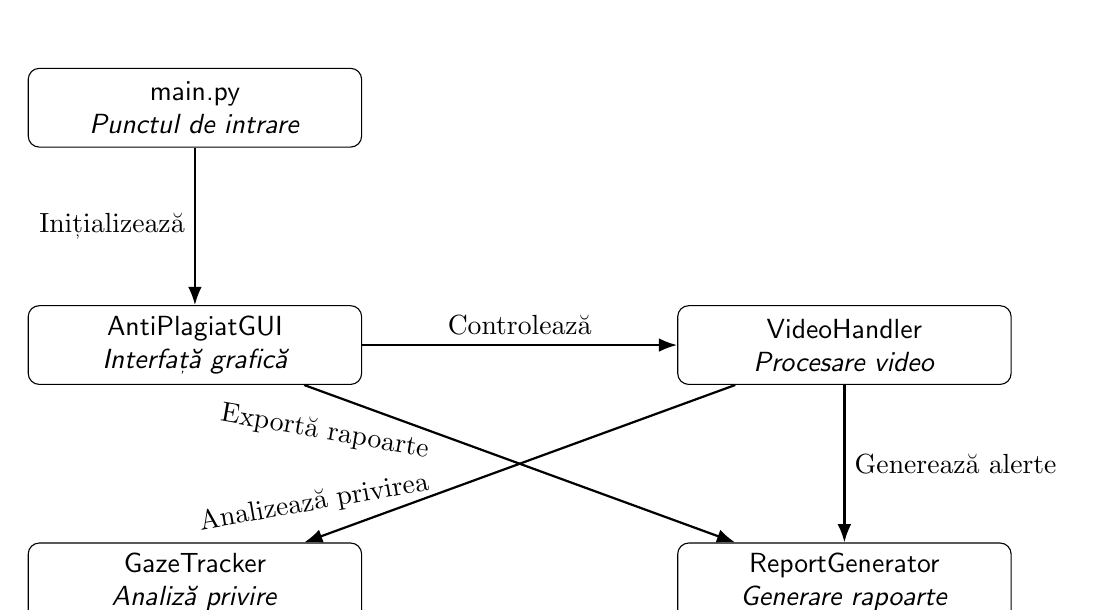
\begin{tikzpicture}[
        class/.style={rectangle, draw=black, rounded corners, text centered, text width=4cm, minimum height=1cm, font=\sffamily},
        relation/.style={-{Latex}, thick},
        aggregation/.style={-{Diamond[open]}, thick},
        composition/.style={-{Diamond}, thick},
        dependency/.style={dashed, -{Latex}, thick}
    ]
        % Classes
        \node[class] (main) {main.py\\\textit{Punctul de intrare}};
        \node[class, below=2cm of main] (gui) {AntiPlagiatGUI\\\textit{Interfață grafică}};
        \node[class, right=4cm of gui] (video) {VideoHandler\\\textit{Procesare video}};
        \node[class, below=2cm of gui] (gaze) {GazeTracker\\\textit{Analiză privire}};
        \node[class, below=2cm of video] (report) {ReportGenerator\\\textit{Generare rapoarte}};

        % Relations
        \draw[relation] (main) -- (gui) node[midway, left] {Inițializează};
        \draw[relation] (gui) -- (video) node[midway, above] {Controlează};
        \draw[relation] (gui) -- (report) node[midway, left, xshift=-1cm, yshift=0.4cm] {\rotatebox{-10}{Exportă rapoarte}};
        \draw[relation] (video) -- (gaze) node[midway, left, xshift=-1cm, yshift=-0.5cm] {\rotatebox{+10}{Analizează privirea}};
        \draw[relation] (video) -- (report) node[midway, right] {Generează alerte};
    \end{tikzpicture}
    \caption{Diagrama de clase a sistemului Anti-Plagiat}
\end{figure}

\subsection{Diagrama de secvență}

\begin{figure}[H]
    \centering
    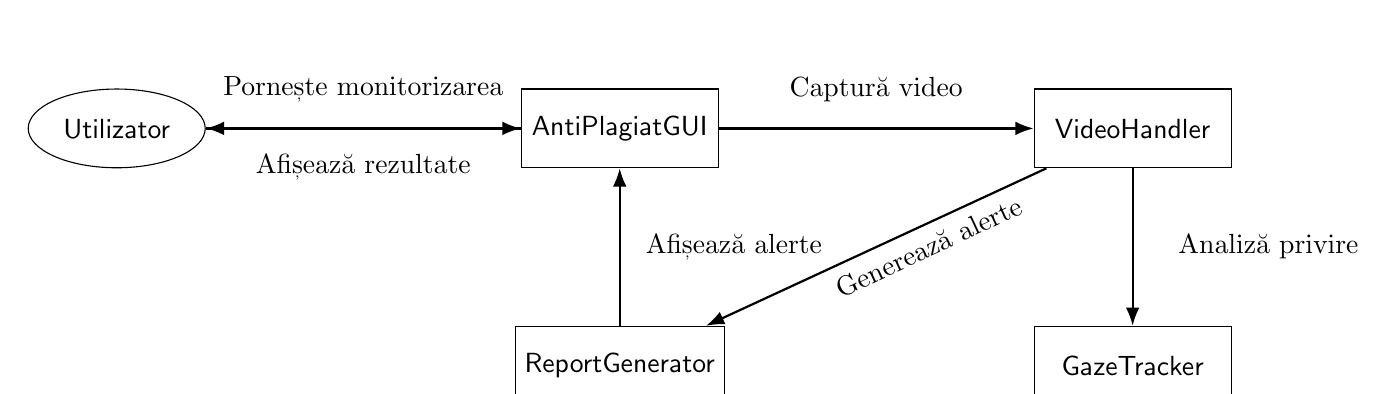
\begin{tikzpicture}[
        actor/.style={draw, ellipse, minimum height=1cm, minimum width=2cm, font=\sffamily},
        process/.style={draw, rectangle, minimum height=1cm, minimum width=2.5cm, font=\sffamily},
        arrow/.style={-{Latex}, thick},
        dashedarrow/.style={dashed, -{Latex}, thick}
    ]
        % Nodes
            \node[actor] (user) {Utilizator};
            \node[process, right=4cm of user] (gui) {AntiPlagiatGUI};
            \node[process, right=4cm of gui] (video) {VideoHandler};
            \node[process, below=2cm of video] (gaze) {GazeTracker};
            \node[process, below=2cm of gui] (report) {ReportGenerator};

            % Arrows
            \draw[arrow] (user) -- (gui) node[midway, above, yshift=0.2cm] {Pornește monitorizarea};
            \draw[arrow] (gui) -- (video) node[midway, above, yshift=0.2cm] {Captură video};
            \draw[arrow] (video) -- (gaze) node[midway, left, xshift=3cm] {Analiză privire};
            \draw[arrow] (video) -- (report) node[midway, right, xshift=-0.68cm] {\rotatebox{+25}{Generează alerte}};
            \draw[arrow] (report) -- (gui) node[midway, right, xshift=0.2cm] {Afișează alerte};
            \draw[dashedarrow] (gui) -- (user) node[midway, below, yshift=-0.2cm] {Afișează rezultate};
    \end{tikzpicture}
    \caption{Diagrama de secvență pentru procesul de detectare a încălcărilor}
\end{figure}

\subsection{Diagrama de activitate}

\begin{figure}[H]
    \centering
    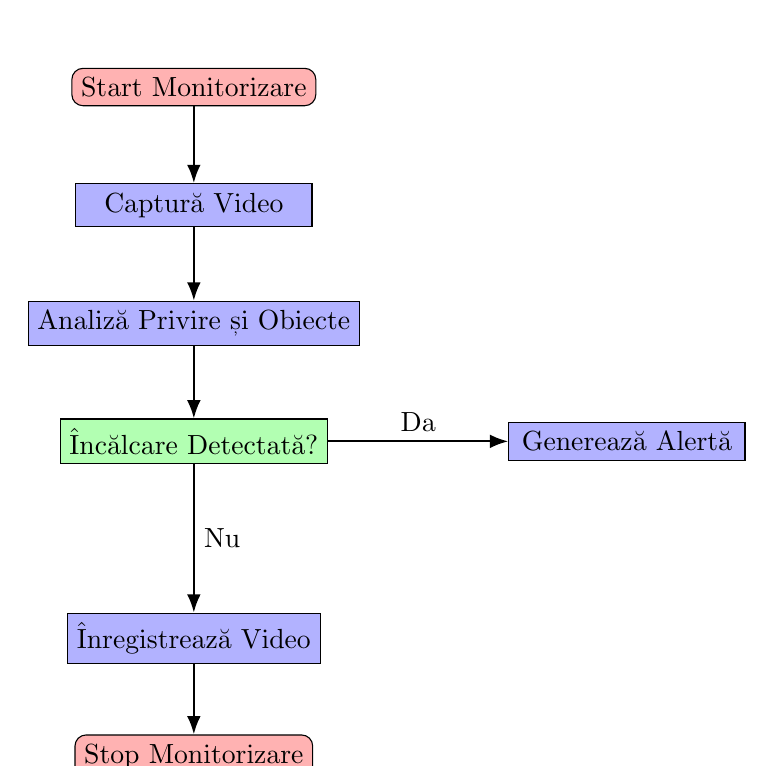
\begin{tikzpicture}[
        node distance=1.5cm,
        startstop/.style={rectangle, rounded corners, draw=black, fill=red!30, text centered, minimum width=3cm},
        process/.style={rectangle, draw=black, fill=blue!30, text centered, minimum width=3cm},
        decision/.style={rectangle, draw=black, fill=green!30, text centered, minimum width=3cm},
        arrow/.style={-{Latex}, thick}
    ]
        % Nodes
        \node[startstop] (start) {Start Monitorizare};
        \node[process, below of=start] (capture) {Captură Video};
        \node[process, below of=capture] (analyze) {Analiză Privire și Obiecte};
        \node[decision, below of=analyze] (violation) {Încălcare Detectată?};
        \node[process, right of=violation, xshift=4cm] (alert) {Generează Alertă};
        \node[process, below of=violation, yshift=-1cm] (record) {Înregistrează Video};
        \node[startstop, below of=record] (stop) {Stop Monitorizare};

        % Arrows
        \draw[arrow] (start) -- (capture);
        \draw[arrow] (capture) -- (analyze);
        \draw[arrow] (analyze) -- (violation);
        \draw[arrow] (violation.east) -- (alert.west) node[midway, above] {Da};
        \draw[arrow] (violation.south) -- (record.north) node[midway, right] {Nu};
        \draw[arrow] (record) -- (stop);
    \end{tikzpicture}
    \caption{Diagrama de activitate pentru procesul de monitorizare}
\end{figure}

\subsection{Diagrama de componente}

\begin{figure}[H]
    \centering
    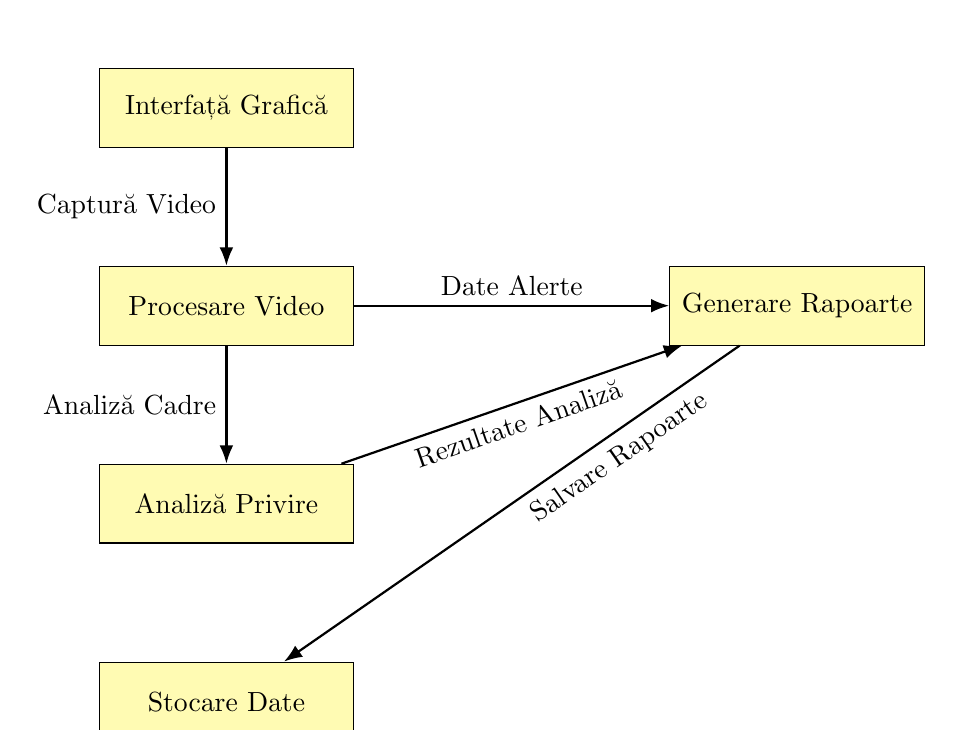
\begin{tikzpicture}[
        component/.style={rectangle, draw=black, fill=yellow!30, text centered, text width=3cm, minimum height=1cm},
        relation/.style={-{Latex}, thick}
    ]
            \node[component] (gui) {Interfață Grafică};
            \node[component, below=1.5cm of gui] (video) {Procesare Video};
            \node[component, below=1.5cm of video] (gaze) {Analiză Privire};
            \node[component, right=4cm of video] (report) {Generare Rapoarte};
            \node[component, below=1.5cm of gaze] (storage) {Stocare Date};

            % Relations
            \draw[relation] (gui) -- (video) node[midway, left] {Captură Video};
            \draw[relation] (video) -- (gaze) node[midway, left] {Analiză Cadre};
            \draw[relation] (video) -- (report) node[midway, above] {Date Alerte};
            \draw[relation] (gaze) -- (report) node[midway, below, sloped, rotate=0] {Rezultate Analiză};
            \draw[relation] (report) -- (storage) node[midway, right, sloped, rotate=0, yshift=-0.3cm] {Salvare Rapoarte};
    \end{tikzpicture}
    \caption{Diagrama de componente a sistemului Anti-Plagiat}
\end{figure}

\section{Dificultăți întâmpinate}

În realizarea acestui proiect, am întâmpinat mai multe dificultăți, care au necesitat soluții creative și adaptări pentru a fi depășite:

\begin{enumerate}
    \item \textbf{Integrarea modelelor YOLOv8:} Configurarea și optimizarea modelelor YOLOv8 pentru detectarea obiectelor interzise a fost o provocare, mai ales în ceea ce privește reducerea falsurilor pozitive. A fost necesar să ajustez pragurile de detecție și să folosesc modele separate pentru categorii diferite de obiecte.

    \item \textbf{Performanța pe hardware limitat:} Procesarea video în timp real a fost dificilă pe dispozitive cu resurse hardware limitate. Am implementat optimizări, cum ar fi procesarea unui cadru din 20 și utilizarea unui buffer circular, pentru a reduce consumul de resurse.

    \item \textbf{Detectarea privirii în condiții de iluminare variabilă:} Detectarea precisă a direcției privirii a fost afectată de variațiile de iluminare. A fost necesar să aplic filtre și să ajusteze parametrii algoritmilor pentru a îmbunătăți robustețea.

    \item \textbf{Sincronizarea datelor multimedia:} Corelarea precisă între fluxul video, audio și evenimentele detectate a fost o sarcină complexă. Am utilizat timestamp-uri sincronizate pentru a lega alertele generate de momentele exacte din fluxul video.

    \item \textbf{Complexitatea interfeței grafice:} Dezvoltarea unei interfețe grafice intuitive și funcționale a fost o provocare, mai ales în ceea ce privește organizarea logică a componentelor și sincronizarea acestora cu procesele din fundal.

    \item \textbf{Gestionarea falsurilor pozitive:} În timpul testării, am observat o rată ridicată de falsuri pozitive, mai ales în detectarea obiectelor. A fost necesar să ajustez algoritmii și să implementez filtre suplimentare pentru a îmbunătăți acuratețea.

    \item \textbf{Documentarea și modularizarea codului:} Structurarea proiectului într-un mod modular și documentarea clară a fiecărui modul au necesitat timp suplimentar, dar au fost esențiale pentru întreținerea și extinderea ulterioară a aplicației.

    \item \textbf{Testarea și validarea:} Testarea aplicației în scenarii reale a fost dificilă, mai ales în simularea condițiilor variate de utilizare, cum ar fi diferite unghiuri ale camerei, iluminare slabă sau zgomot de fundal.

    \item \textbf{Gestionarea dependențelor:} Instalarea și configurarea corectă a tuturor bibliotecilor și pachetelor necesare au fost uneori problematice, mai ales din cauza incompatibilităților între versiuni.
\end{enumerate}

Aceste dificultăți au reprezentat oportunități de învățare și au contribuit la îmbunătățirea abilităților mele tehnice și de gestionare a proiectelor.

\section{Contribuția personală}

În cadrul acestui proiect, am adus mai multe contribuții semnificative, care includ:

\subsection{Utilizarea a două modele YOLOv8 pentru detectarea obiectelor interzise}
Am utilizat două modele YOLOv8 separate, unul specializat pentru detectarea telefoanelor mobile și altul pentru detectarea smartwatch-urilor. Această abordare a fost aleasă pentru a lucra eficient și pentru a elimina falsurile pozitive. În loc să reantrenăm un model unic pentru ambele categorii, am aplicat clasificări stricte bazate pe dimensiunile \textit{x-y} ale obiectelor detectate.

\textbf{Exemplu din cod:}
\begin{lstlisting}[language=Python]
# filepath: /home/valentin/Desktop/anti-plagiat/modules/video_handler.py
if detection["class"] == "phone" and detection["width"] > 50:
    process_phone_detection(detection)
elif detection["class"] == "smartwatch" and detection["width"] <= 50:
    process_smartwatch_detection(detection)
\end{lstlisting}

\subsection{Implementarea calculelor de algebră liniară pentru analiza privirii}
Am dezvoltat și integrat calcule de algebră liniară pentru a determina direcția privirii utilizatorului. Aceste calcule includ:
\begin{itemize}
    \item Determinarea coordonatelor pupilelor utilizând vectori și puncte de referință.
    \item Calcularea raporturilor orizontale și verticale (\textit{horizontal ratio} și \textit{vertical ratio}) pentru a estima direcția privirii.
    \item Filtrarea și ajustarea valorilor pentru a elimina zgomotul și variațiile neașteptate.
\end{itemize}

\textbf{Exemplu din cod:}
\begin{lstlisting}[language=Python]
# filepath: /home/valentin/Desktop/anti-plagiat/modules/gaze_tracking/gaze_tracker.py
pupil_left = self.eye_left.pupil.x / (self.eye_left.center[0] * 2 - 10)
pupil_right = self.eye_right.pupil.x / (self.eye_right.center[0] * 2 - 10)
pupil_ratio = (pupil_left + pupil_right) / 2
\end{lstlisting}

\subsection{Optimizarea procesării video în timp real}
Am implementat optimizări pentru procesarea video, inclusiv:
\begin{itemize}
    \item Procesarea unui cadru din 20 pentru detectarea obiectelor, reducând astfel consumul de resurse.
    \item Utilizarea unui buffer circular pentru gestionarea eficientă a cadrelor video.
    \item Integrarea unui sistem de cache pentru alertele generate, evitând duplicarea mesajelor de alertă.
\end{itemize}

\textbf{Exemplu din cod:}
\begin{lstlisting}[language=Python]
# filepath: /home/valentin/Desktop/anti-plagiat/modules/video_handler.py
if self.frame_count % 20 == 0:
    detections = self.model.predict(frame)
\end{lstlisting}

\subsection{Generarea rapoartelor detaliate}
Am dezvoltat un sistem de generare automată a rapoartelor în formate HTML, CSV și JSON. Aceste rapoarte includ:
\begin{itemize}
    \item Timpul exact al fiecărei încălcări detectate.
    \item Tipul obiectului detectat și locația acestuia în cadrul video.
    \item Rezumatul general al sesiunii de monitorizare.
\end{itemize}

\textbf{Exemplu din cod:}
\begin{lstlisting}[language=Python]
# filepath: /home/valentin/Desktop/anti-plagiat/modules/report_generator.py
<p>Total incalcari detectate: <strong>{total_violations}</strong></p>
<p>Durata monitorizare: De la {violation_log[0]["timestamp"]} pana la {violation_log[-1]["timestamp"]}</p>
\end{lstlisting}

\subsection{Integrarea interfeței grafice intuitive}
Am dezvoltat o interfață grafică intuitivă utilizând PyQt5, care permite utilizatorilor să:
\begin{itemize}
    \item Pornească și oprească monitorizarea în timp real.
    \item Vizualizeze alertele generate în timp real.
    \item Exporte rapoarte detaliate cu un singur clic.
\end{itemize}

\textbf{Exemplu din cod:}
\begin{lstlisting}[language=Python]
# filepath: /home/valentin/Desktop/anti-plagiat/gui_app.py
self.export_button = QPushButton("Export Raport")
self.export_button.clicked.connect(self.export_report)
\end{lstlisting}

\section{Îmbunătățiri posibile}

Deși aplicația actuală oferă funcționalități avansate pentru monitorizarea anti-plagiat, există câteva aspecte care pot fi îmbunătățite sau extinse pentru a crește eficiența și utilitatea acesteia:

\begin{enumerate}
    \item \textbf{Integrarea cu platforme LMS:} Adăugarea suportului pentru integrarea directă cu platforme de management al învățământului (LMS), precum Moodle, Blackboard sau Canvas, pentru a facilita gestionarea examenelor și a rapoartelor.

    \item \textbf{Detectarea comportamentului complex:} Utilizarea modelelor avansate de machine learning pentru a analiza comportamente mai complexe, cum ar fi mișcările subtile ale mâinilor sau schimbările de expresie facială.

    \item \textbf{Suport multi-camera:} Extinderea aplicației pentru a permite utilizarea mai multor camere simultan, oferind o perspectivă mai completă asupra comportamentului candidatului.

    \item \textbf{Reducerea falsurilor pozitive:} Îmbunătățirea algoritmilor de detecție pentru a reduce rata falsurilor pozitive, prin utilizarea unor modele mai bine antrenate sau prin combinarea mai multor surse de date.

    \item \textbf{Monitorizare audio avansată:} Dezvoltarea unui modul de procesare audio mai sofisticat, care să detecteze conversațiile suspecte sau utilizarea dispozitivelor audio neautorizate.

    \item \textbf{Suport pentru dispozitive mobile:} Crearea unei versiuni a aplicației care să funcționeze pe dispozitive mobile, pentru a extinde utilizarea acesteia în medii mai diverse.

    \item \textbf{Personalizarea interfeței grafice:} Adăugarea opțiunilor de personalizare a interfeței grafice, cum ar fi temele de culoare sau configurarea widget-urilor, pentru a îmbunătăți experiența utilizatorului.

    \item \textbf{Analiză post-eveniment:} Dezvoltarea unui modul avansat de analiză post-eveniment, care să permită revizuirea detaliată a sesiunilor de monitorizare, cu funcționalități precum căutarea pe baza timestamp-urilor sau generarea de grafice.

    \item \textbf{Optimizări hardware:} Implementarea unor optimizări suplimentare pentru a reduce consumul de resurse pe dispozitive cu hardware limitat, cum ar fi utilizarea procesării GPU sau a modelelor mai ușoare.
\end{enumerate}

Aceste îmbunătățiri ar putea crește semnificativ valoarea aplicației și ar extinde aria de utilizare a acesteia în diverse contexte educaționale și profesionale.

\begin{thebibliography}{9}
\bibitem{pelican} 
Pelican, G. (2021) 
\textit{Plagiatul - o plagă academică endemică}. 
\url{https://inm-lex.ro/wp-content/uploads/2021/12/Pelican-G-Plagiatul-o-plaga-academica-endemica.pdf}

\bibitem{science} 
Science (2018)
\textit{What a massive database of retracted papers reveals about science publishing's 'death penalty'}.
\url{https://www.science.org/content/article/what-massive-database-retracted-papers-reveals-about-science-publishing-s-death-penalty}

\bibitem{proctoru} 
ProctorU Official Website. 
\url{https://www.proctoru.com/}

\bibitem{proctorio} 
Proctorio Official Website. 
\url{https://proctorio.com/}

\bibitem{respondus} 
Respondus LockDown Browser Documentation. 
\url{https://web.respondus.com/lockdownbrowser/}

\bibitem{opencv} 
OpenCV Documentation. 
\url{https://opencv.org/}

\bibitem{dlib} 
Dlib Documentation. 
\url{http://dlib.net/}

\bibitem{pytorch} 
PyTorch Documentation. 
\url{https://pytorch.org/}

\bibitem{ultralytics} 
Ultralytics YOLOv8 Documentation. 
\url{https://github.com/ultralytics/ultralytics}

\bibitem{numpy} 
NumPy Documentation. 
\url{https://numpy.org/}

\bibitem{pyqt5} 
PyQt5 Documentation. 
\url{https://riverbankcomputing.com/software/pyqt/intro}

\bibitem{datetime} 
Python datetime Module Documentation. 
\url{https://docs.python.org/3/library/datetime.html}

\bibitem{logging} 
Python logging Module Documentation. 
\url{https://docs.python.org/3/library/logging.html}
\end{thebibliography}

\end{document}